
%%%%%%%%%%%%%%%%%%%%%%%%%%%%%%%%%%%%%%%%%%%%%%%%%%%%%%%%%%%%%%%%%%%%%
%% This is a (brief) model paper using the achemso class
%% The document class accepts keyval options, which should include
%% the target journal and optionally the manuscript type.
%%%%%%%%%%%%%%%%%%%%%%%%%%%%%%%%%%%%%%%%%%%%%%%%%%%%%%%%%%%%%%%%%%%%%
\documentclass[journal=apchd5,manuscript=article]{achemso}

%%%%%%%%%%%%%%%%%%%%%%%%%%%%%%%%%%%%%%%%%%%%%%%%%%%%%%%%%%%%%%%%%%%%%
%% Place any additional packages needed here.  Only include packages
%% which are essential, to avoid problems later. Do NOT use any
%% packages which require e-TeX (for example etoolbox): the e-TeX
%% extensions are not currently available on the ACS conversion
%% servers.
%%%%%%%%%%%%%%%%%%%%%%%%%%%%%%%%%%%%%%%%%%%%%%%%%%%%%%%%%%%%%%%%%%%%%
\usepackage[version=3]{mhchem} % Formula subscripts using \ce{}
\usepackage[T1]{fontenc}       % Use modern font encodings
\usepackage{graphicx}
\usepackage{amsmath}
\usepackage{xcolor}
\usepackage{wrapfig}
%%%%%%%%%%%%%%%%%%%%%%%%%%%%%%%%%%%%%%%%%%%%%%%%%%%%%%%%%%%%%%%%%%%%%
%% If issues arise when submitting your manuscript, you may want to
%% un-comment the next line.  This provides information on the
%% version of every file you have used.
%%%%%%%%%%%%%%%%%%%%%%%%%%%%%%%%%%%%%%%%%%%%%%%%%%%%%%%%%%%%%%%%%%%%%
%%\listfiles

%%%%%%%%%%%%%%%%%%%%%%%%%%%%%%%%%%%%%%%%%%%%%%%%%%%%%%%%%%%%%%%%%%%%%
%% Place any additional macros here.  Please use \newcommand* where
%% possible, and avoid layout-changing macros (which are not used
%% when typesetting).
%%%%%%%%%%%%%%%%%%%%%%%%%%%%%%%%%%%%%%%%%%%%%%%%%%%%%%%%%%%%%%%%%%%%%
\newcommand*\mycommand[1]{\texttt{\emph{#1}}}

%%%%%%%%%%%%%%%%%%%%%%%%%%%%%%%%%%%%%%%%%%%%%%%%%%%%%%%%%%%%%%%%%%%%%
%% Meta-data block
%% ---------------
%% Each author should be given as a separate \author command.
%%
%% Corresponding authors should have an e-mail given after the author
%% name as an \email command. Phone and fax numbers can be given
%% using \phone and \fax, respectively; this information is optional.
%%
%% The affiliation of authors is given after the authors; each
%% \affiliation command applies to all preceding authors not already
%% assigned an affiliation.
%%
%% The affiliation takes an option argument for the short name.  This
%% will typically be something like "University of Somewhere".
%%
%% The \altaffiliation macro should be used for new address, etc.
%% On the other hand, \alsoaffiliation is used on a per author basis
%% when authors are associated with multiple institutions.
%%%%%%%%%%%%%%%%%%%%%%%%%%%%%%%%%%%%%%%%%%%%%%%%%%%%%%%%%%%%%%%%%%%%%
\author{Nicholas P. Montoni}
\author{Steven C. Quillin}
\author{Charles Cherqui}
\affiliation[Department of Chemistry, University of Washington]
{Department of Chemistry, University of Washington, Seattle, WA 98195}
\author{David J. Masiello}
\affiliation[Department of Chemistry, University of Washington]
{Department of Chemistry, University of Washington, Seattle, WA 98195}
\alsoaffiliation[Department of Applied Mathematics, University of Washington]
{Department of Applied Mathematics, University of Washington, Seattle, WA 98195}
\email{masiello@chem.washington.edu}

%%%%%%%%%%%%%%%%%%%%%%%%%%%%%%%%%%%%%%%%%%%%%%%%%%%%%%%%%%%%%%%%%%%%%
%% The document title should be given as usual. Some journals require
%% a running title from the author: this should be supplied as an
%% optional argument to \title.
%%%%%%%%%%%%%%%%%%%%%%%%%%%%%%%%%%%%%%%%%%%%%%%%%%%%%%%%%%%%%%%%%%%%%
\title[]
    {Towards Tunable Negative-Index Metamaterials}
%%%%%%%%%%%%%%%%%%%%%%%%%%%%%%%%%%%%%%%%%%%%%%%%%%%%%%%%%%%%%%%%%%%%%
%% Some journals require a list of abbreviations or keywords to be
%% supplied. These should be set up here, and will be printed after
%% the title and author information, if needed.
%%%%%%%%%%%%%%%%%%%%%%%%%%%%%%%%%%%%%%%%%%%%%%%%%%%%%%%%%%%%%%%%%%%%%
\abbreviations{MNP, LSPR, EELS}
\keywords{plasmon, hybridization, magnetic, retardation}

%%%%%%%%%%%%%%%%%%%%%%%%%%%%%%%%%%%%%%%%%%%%%%%%%%%%%%%%%%%%%%%%%%%%%
%% The manuscript does not need to include \maketitle, which is
%% executed automatically.
%%%%%%%%%%%%%%%%%%%%%%%%%%%%%%%%%%%%%%%%%%%%%%%%%%%%%%%%%%%%%%%%%%%%%
\begin{document}

%%%%%%%%%%%%%%%%%%%%%%%%%%%%%%%%%%%%%%%%%%%%%%%%%%%%%%%%%%%%%%%%%%%%%
%% The "tocentry" environment can be used to create an entry for the
%% graphical table of contents. It is given here as some journals
%% require that it is printed as part of the abstract page. It will
%% be automatically moved as appropriate.
%%%%%%%%%%%%%%%%%%%%%%%%%%%%%%%%%%%%%%%%%%%%%%%%%%%%%%%%%%%%%%%%%%%%%
\begin{tocentry}

Some journals require a graphical entry for the Table of Contents.
This should be laid out ``print ready'' so that the sizing of the
text is correct.

Inside the \texttt{tocentry} environment, the font used is Helvetica
8\,pt, as required by \emph{Journal of the American Chemical
Society}.

The surrounding frame is 9\,cm by 3.5\,cm, which is the maximum
permitted for  \emph{Journal of the American Chemical Society}
graphical table of content entries. The box will not resize if the
content is too big: instead it will overflow the edge of the box.

This box and the associated title will always be printed on a
separate page at the end of the document.

\end{tocentry}

%%%%%%%%%%%%%%%%%%%%%%%%%%%%%%%%%%%%%%%%%%%%%%%%%%%%%%%%%%%%%%%%%%%%%
%% The abstract environment will automatically gobble the contents
%% if an abstract is not used by the target journal.
%%%%%%%%%%%%%%%%%%%%%%%%%%%%%%%%%%%%%%%%%%%%%%%%%%%%%%%%%%%%%%%%%%%%%
\begin{abstract}
Ring-like assemblies of metal nanoparticles that exhibit magnetic resonances, called magentic plasmon oligomers, have been of recent interest as negative-index metamaterials. Magnetic plasmon oligomers have potential applications in cloaking, superlensing, information transmission, and sensing. For these reasons, it is imperative to understand the properties of such systems on both small and large scales. We show through theory and simulation that the energy ordering of the magnetic resonances of small oligomers depends greatly on the size and scale of the nanoparticle assembly in ways that purely electric plasmons do not. Following this, we determine the effective pemeability and permittivity of periodic arrays of nanoparticles and show that in certain size regimes they exhibit a negative index of refraction at optical frequencies. As a final exercise, we propose a negative-index material composed of charge tunable semiconductor quantum dots to emphasize the direct control of the optical properties of 2-D magnetic materials.
\end{abstract}

%%%%%%%%%%%%%%%%%%%%%%%%%%%%%%%%%%%%%%%%%%%%%%%%%%%%%%%%%%%%%%%%%%%%%
%% Start the main part of the manuscript here.
%%%%%%%%%%%%%%%%%%%%%%%%%%%%%%%%%%%%%%%%%%%%%%%%%%%%%%%%%%%%%%%%%%%%%
\section{Introduction}
Bringing two or more metal nanoparticles (MNPs) together allows their individual electric plasmons to hybridize, producing a new set of plasmonic modes\cite{Lucas1976,ARAVIND1981,Xu1995,Mischenko1995}. Plasmon hybridization theory is applied to aggregates of MNPs and explains their collective behavior within the quasistatic limit in which the speed of light is taken to be infinite\cite{NordHal2003,NordProdan2004,Oubre2004,Gomez2009}. Recently, retardation effects on plasmon hybridization have been the focus of study for large particles\cite{Abajo2008,Gu2010} as well as dimers\cite{vonPlessen2007,Rechbacher2003,Kottman2001}, and 2-D arrays\cite{Schatz2003,Royer2005,Chumanov2010} of nanoparticles. Specific arrangements of nanoparticles in 2-D arrays, such as three or more nanoparticles arranged on the vertices of a regular polygon, support a collective mode in which all of the dipole plasmons are oriented head-to-tail. This generates a fictitious, oscillating current loop resulting in an oscillating magnetic dipole moment in the center of the ring\cite{Alu2006,Alu2008,Liu2011,Nord2006,Cherqui2014,Cherqui2016}. These so-called magnetic plasmons are the lowest-energy collective modes of the oligomers and couple to and enhance the magnetic field of incident light\cite{Shalaev2007,Qian2015,Nord2007}, offering a route to applications such as solar cell enhancement\cite{Graydon2011,Alu2014solar,Le2015solar}, biosensing and detection\cite{Zia2010trans,Noginova2008trans,Wang:13,Fan2015,Wei2015,Shvets2012,Altug2012bio,Nord2011fano}, and information storage and propagation\cite{Zhang2006,NordHal2011,NordHal2012}. The rich plasmonic modes of magnetic-plasmon-supporting systems are well-described using plasmon hybridization theory, but when in the quasistatic limit, the energy-order of the modes is not.

Plasmon hybridization theory treats plasmons as point dipoles centered on their associated nanoparticles that interact through dipole-dipole coupling. In the quasistatic limit, these dipoles couple only through time-independent, electric near-field interactions\cite{jackson_classical_1999}, but when the size of and distance between nanoparticles becomes large, this approximation breaks down and intermediate- and far-field effects must be considered, as well as time-delay effects in the near-field\cite{jackson_classical_1999}. The aim of this paper is to incorporate the fully retarded electric field into plasmon hybridization theory and extend studies of retardation effects to magnetic plasmon oligomers. Specifically, we begin by exploring oligomers comprising two and three rings of nanoparticles and compare to full-wave simulation \cite{Hohenester2012} to verify that our approach qualitatively predicts the energy-ordering of the magnetic modes.\cite{Cherqui2014,Cherqui2016}. Following this, we calaculate the coupling betwen individual rings in various oligomers in order to parametrize an effective magnetic-magnetic coupling between magnetic dipoles. Using this new basis, we describe periodic chains and arrays of oligomers.

The calculations presented here are performed using an electric tight-binding model, parametrizing the magnetic couplings, and then introducing these coupling constants into a magnetic tight-binding model. For all following magnetic oligomers, only the two planar dipoles per particle are considered in the electric tight binding model. The dipoles are mapped onto a set of harmonic oscillators and are described by the following Hamiltonian:

\begin{equation}
H = \sum_{i}^{n}\frac{\textbf{P}_{i}^{2}}{2m_{\textrm{sp},i}} + \frac{1}{2}m_{\textrm{sp},i}w_{\textrm{sp},i}^2\textbf{X}_{i}^{2} + e^2\sum_{i\neq j}\textbf{X}_i\cdot\boldsymbol{\Lambda}_{\textrm{full},ij}\cdot\textbf{X}_j,\label{elec_hammy_1}
\end{equation}

where $\textbf{P}_i$ are the momenta conjugate to the coordinates $\textbf{X}_{i}$, $\omega_{sp,i}$ are the individual LSPR frequencies of each oscillator, $m_{sp,i}$ are the LSPR effective masses and $\boldsymbol{\Lambda}_{\textrm{full},ij}$ is the fully retarded dipole-dipole relay tensor (expanded below). To make this Hamiltonian more manageable, it is nondimensionalized using $\textbf{Q}_i = \left(m_{\textrm{sp}}\omega_{\textrm{sp}}/\hbar\right)^{\frac{1}{2}}\textbf{X}_i$ and $\boldsymbol{\Pi}_i = \textbf{P}_i/\sqrt{\hbar m_{\textrm{sp}}\omega_{\textrm{sp}}}$. Substituting into Equation~\ref{elec_hammy_1} and expanding $\boldsymbol{\Lambda}_{\textrm{full},ij}$, we get:

\begin{equation}
\begin{aligned}
H = 
\frac{\hbar\omega_{sp}}{2}\sum_{i}^{n}[\boldsymbol{\Pi}_i^2 + \textbf{Q}_i^2] - \frac{\hbar\omega_{sp}}{2}\sum_{i\neq j}\{g_{ij}^{\textrm{NF}}\left[3(\textbf{Q}_i\cdot\hat{\textbf{n}}_{ij})(\hat{\textbf{n}}_{ij}\cdot\textbf{Q}_j) - \textbf{Q}_i\cdot\textbf{Q}_j\right] \\
+ g_{ij}^{\textrm{IF}}\left[3(\textbf{Q}_i\cdot\hat{\textbf{n}}_{ij})(\hat{\textbf{n}}_{ij}\cdot\textbf{Q}_j) -\textbf{Q}_i\cdot\textbf{Q}_j\right] \\ 
- g_{ij}^{\textrm{FF}}\left[(\textbf{Q}_i\cdot\hat{\textbf{n}}_{ij})(\hat{\textbf{n}}_{ij}\cdot\textbf{Q}_j) -\textbf{Q}_i\cdot\textbf{Q}_j\right]\},\label{elec_hammy_2}
\end{aligned}
\end{equation}

In this Hamiltonian we introduce the near, intermediate, and far-field coupling terms: $g_{ij}^{\textrm{NF}} = \frac{\alpha_{sp}}{r_{ij}^3}\cos\left(\frac{\omega r_{ij}}{c}\right)$, $g_{ij}^{\textrm{IF}} = \frac{\alpha_{sp}\omega}{r_{ij}^2 c}\sin\left(\frac{\omega r_{ij}}{c}\right)$, and $g_{ij}^{\textrm{FF}} = \frac{\alpha_{sp}\omega^2}{r_{ij} c^2}\cos\left(\frac{\omega r_{ij}}{c}\right)$, respectively. Additionally, the polarizability $\alpha_{sp} = \frac{e^2}{m_{sp}\omega_{sp}^2}$, $r_{ij}$ is the distance between the ith and jth LSPs, and $\hat{\textbf{n}}_{ij}$ is the unit vector connecting two LSPs. Including these terms, we have incorporated all retardation effects associated with point dipoles\cite{Purcell1973}.

It should be noted that this Hamiltonian, when diagonilzed, results in a transcendental equation. The eigenvalues of the Hamiltonian are functions of $\omega$, which are the frequencies of the collective modes, that is, the eigenvalues of the eigenvectors. In order to fully solve this problem, we make a first guess of $\omega$ for a particular mode of interest and iteratively compute the eigenvalues. Using the eigenvalue associated with the mode of interest, the Hamiltonian is diagonalized to convergence. The process is repeated for each mode of interest.

\section{results and discussion}
The first systems we examine are a magnetic dimer\cite{Cherqui2014}, a three-ring chain, and three rings arranged in a triangle. Because we are interested in the effects of scale, we must define a scaling parameter for the system. Each of our systems begins from a unit cell: six silver, spherical MNPs placed at the corners of a regular hexagon. To create the dimer, two unit cells are tiled so that they share an edge, and thus two particles. In general, if any two unit cells share an edge, they also share two nanoparticles, as in the diagrams in Figure~\ref{theory_simul} Each particle has radius $a_0$ and particles are separated by lattice spacing $r=2.2\times a_0$. With the radius of the particles defining the scale of the system, there now exists a way to probe the energy ordering of the modes as a function of size.

\begin{figure}
\begin{center}
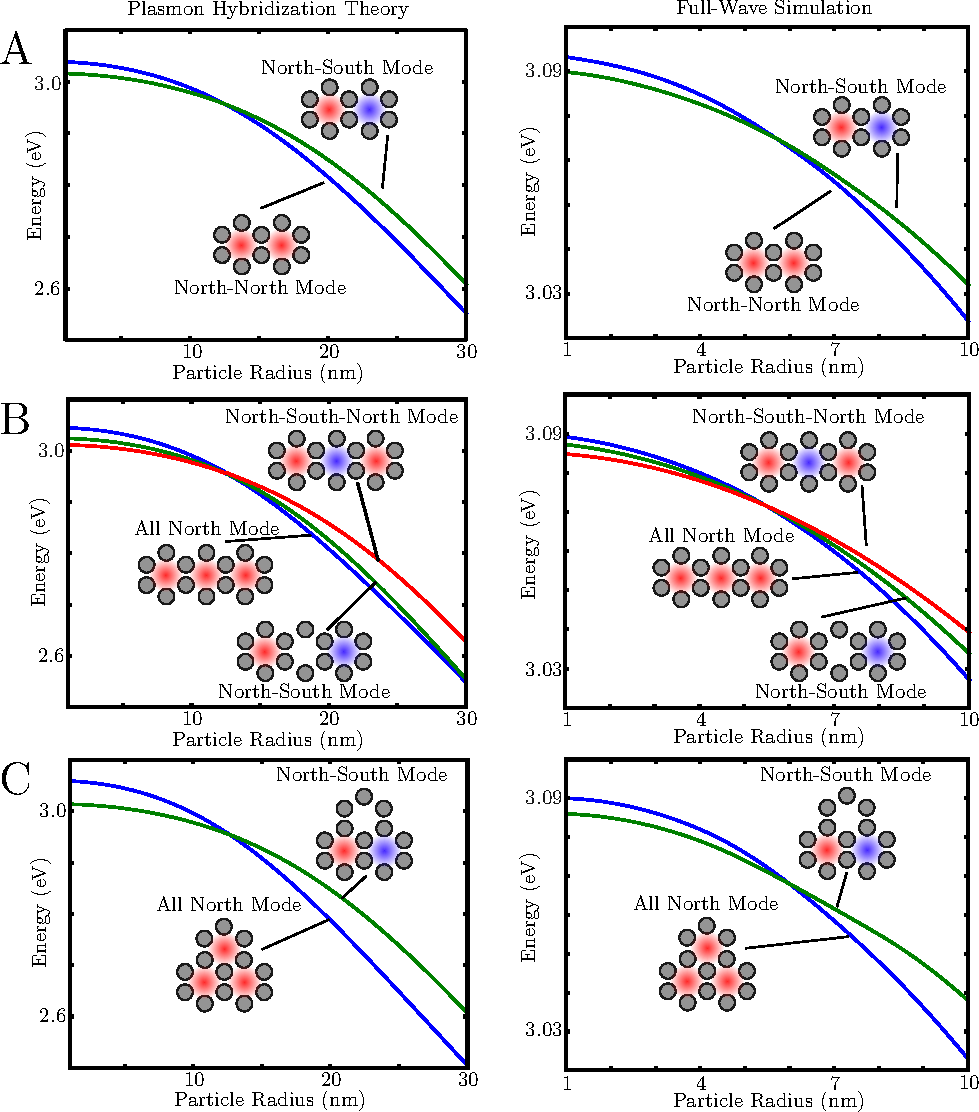
\includegraphics{theory_bem_comparison_fig1.pdf}
\caption{Pending.}
\label{theory_simul}
\end{center}
\end{figure}

The results of our theoretical calculations and full-wave simulations for the aforementioned oligomers are dispayed in Figure~\ref{theory_simul}. Both theory and simulation predict that as a function of size, the energy ordering of the magnetic plasmon modes should change. In the dimer system, there are two magnetic modes. When the system is small, the lowest energy mode is the alternating north-south (NS) mode and the in-phase north-north mode is highest. When we add a ring to the system, we see a trend emerge. The alternating (NSN) mode is lower than the N-S mode, which is in turn lower than the NNN mode. As a function of size, the modes change order. The triangle system, as a result of its threefold symmetry (as opposed to twofold for the chains) has slightly different properties. At small size, its lowest energy mode is a pair of degenerate NS modes, while its higher energy mode is an all-north mode. These again switch order as a function of size. In chains with more than three rings, the pattern continues - the magnetic resonances with the most nodes between rings are the lowest energy when small, but the highest when large.

\begin{figure}
\begin{center}
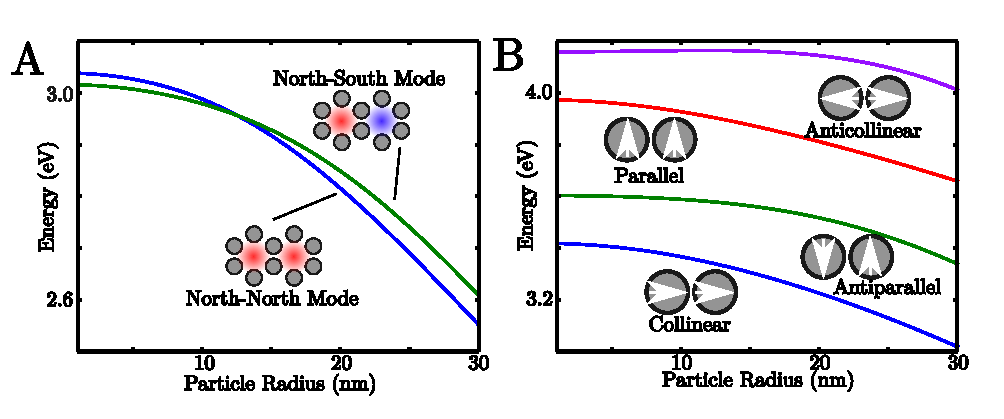
\includegraphics{twomer_dimer.pdf}
\caption{Pending.}
\label{twomer_dimer}
\end{center}
\end{figure}

This is an unexpected phenomenon. When one considers the energy-order of the four (six) hybridized modes of the nanosphere dimer, it becomes clear that they do not exhibit this effect (Figure~\ref{twomer_dimer}). Notably, the sphere dimer shows no crossings while the oligomer dimer does. The reason for this outcome is the oligomer dimer's complex structure\cite{Cherqui2016}. The sphere dimer has only one length scale and consitutes only one pairwise interaction. However, the oligomer dimer contains many pairs of nanoparticles over multiple length scales. As a result, different configurations of electric dipoles will be favored at different oligomer sizes, hence the flip of the magnetic modes.

\begin{figure}
\begin{center}
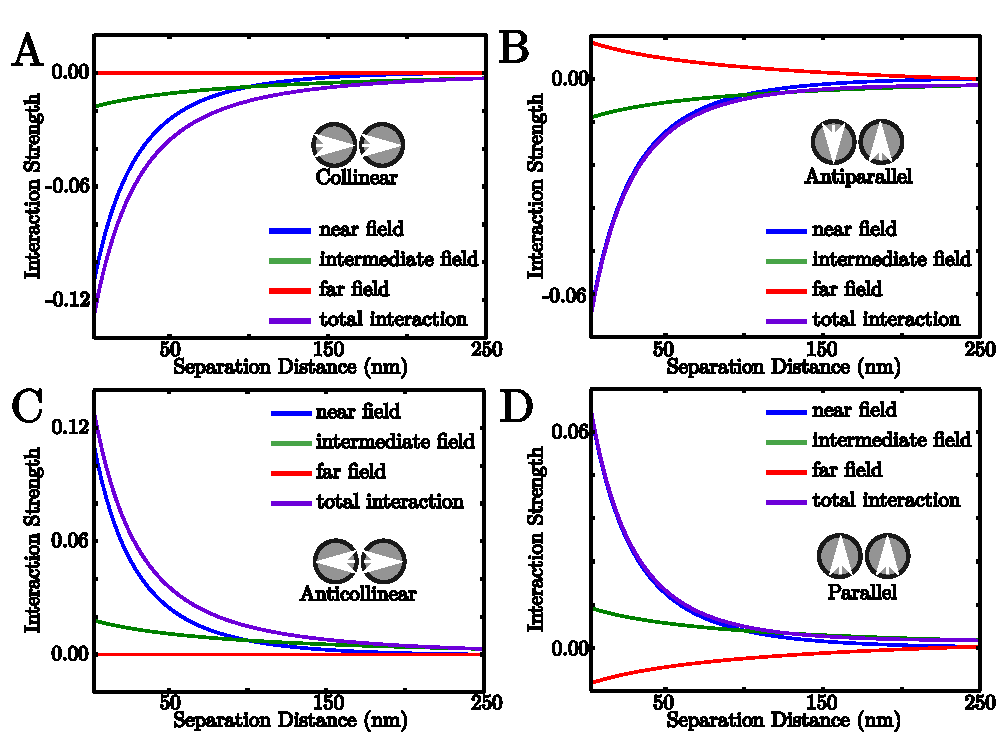
\includegraphics{interactions.pdf}
\caption{Pending.}
\label{int_strength}
\end{center}
\end{figure}

To gain a more visual and intuitive sense of the length scales of each of the terms (near, intermediate, and far) in the fully retarded electric field of a dipole (found in the coupling terms of Equation~\ref{elec_hammy_2}), we calculated the relative interaction strength between pairs of dipoles (the collective modes of the sphere dimer) as a function of dipole separation distance. The results of these calculations are displayed in Figure~\ref{int_strength}, showing that at different length scales, different terms in the field contribute more to the energy of the system. Significantly, the interaction strengths display oscillatory motion, which confirms and reinforces past studies on the oscillatory nature of radiation damping.\cite{vonPlessen2007}

\begin{figure}
\begin{center}
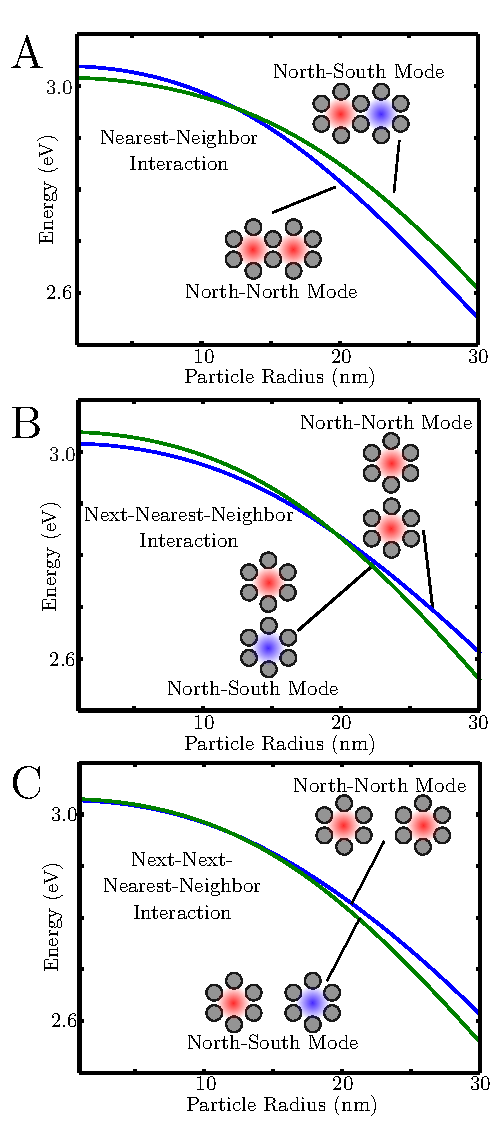
\includegraphics{coupling_comparison.pdf}
\caption{Pending.}
\label{ring_spacing}
\end{center}
\end{figure}

With a functional and accurate electric dipole tight binding model, we seek a way to simplify our model. Figure~\ref{ring_spacing} displays the eigenvalue curves for three arrangements of two-ring systems, with the rings as (A) nearest neighbors (B) next-nearest neighbors and (C) next-next-nearest neighbors. It is clear that again, at different length scales and relative orientations, the eigenvalue curves behave differently, having different crossing points and energy ordering. Using these eigenvalue curves, the electric dipole model is transformed into a magnetic dipole model. A magnetic dipole is placed at the center of each ring with orientation perpendicular to the plane of the ring. Each dipole has natural frequency $\omega_{\textrm{M}}$, which we determine using the electric tight-binding model for a single ring. The coupling between each magnetic dipole is pulled from the plots in figure (w/e) - depending on the spacing between the rings, the dipoles couple through nearest, next-nearest, or next-next-nearest neighbor coupling. The Hamiltonian

\begin{equation}
H = \frac{\hbar\omega_{\textrm{M}}}{2}\sum_{i}^{n}[\pi_{i}^{2}+q_{i}^{2}]+\frac{\hbar\omega_{\textrm{M}}}{2}\sum_{i\neq j}g_{ij}^{\textrm{M}}q_{i}q_{j}
\label{mag_hammy}
\end{equation}

is used in the same way as Equation~\ref{elec_hammy_2} - diagonalizing it for a set of $n$ magnetic dipoles produces $n$ collective magnetic modes. The benefit of this model is shown by example. For the oligomer dimer, there are ten MNPs, each with two electric dipoles, resulting in twenty collectivel electric modes, two of which were magnetic in character. In the magnetic dipole basis, because there are two rings, there are only two modes - the magnetic modes. This simplifies the data analysis procedures greatly. We find that when the couplings between rings are parametrized by the differences between the eigenvalues of the dimers in figure (whatever), the magnetic dipole Hamiltonian reproduces the results of the electric dipole Hamiltonian exactly. We find, furthermore, that truncating to nearest or next-nearest neighbors in the magnetic dipole model does not lead to any significant loss in quantitative or qualitative agreement between the models. It is this finding that will allow us the extension of the model to larger systems considering only nearest or next-nearest neigbor coupling.

The significant challenge here is to find a colloquial, qualitative, and accurate way to describe extended systems. By considering the magnetic dimer to be a unit cell of extended systems, the path to characterizing large systems is through a method similar to a two-atom basis molecular tight-binding model. Here, however, the atoms are the rings of the dimer, and the elements of the hopping matrix are determined by the inter-ring couplings calculated above. More on this model will be presented later.

\section{Dielectric Background and a Measure of Quasistaticity}

As an additional exercise, and to emphasize the tunability and versatility of magnetic plasmon oligomers, the effect of the dielectric constant of the background ($\varepsilon_{b}$) is also taken into account. The dielectric constant screens the electric dipoles from each other by effectively weakening their induced electric fields. This means that as $\varepsilon_{b}$ gets large, intermediate and far field effects will weaken in comparison to near field contributions to the electric field. Thus, magnetic plasmon oligomers will be more likely to behave quasistatically when large. In Figure~\ref{diel_eff}A, the difference between the NN and NS modes for magnetic dimers of four different scaling factors embedded in media with $\varepsilon_{b} = 1$ to $10$ are presented as an example of the impact of screening on the energy ordering of magnetic modes. The results show that when highly screened, even large magnetic plasmon oligomers behave quasistatically.

\begin{figure}
\begin{center}
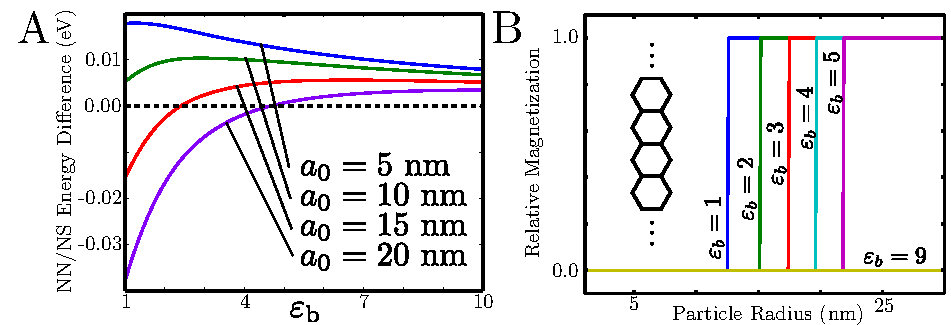
\includegraphics{diel_magnetization.pdf}
\caption{Pending.}
\label{diel_eff}
\end{center}
\end{figure}

To extend this to a potential application, we consider now a periodic chain of magnetic monomers - essentially a 1-D system - with only nearest neighbor coupling. When the radii of the particles in the chain are small, the lowest energy collective mode of the chain will be an all-alternating magnetic mode, and when the radii are large it will be an all in-phase magnetic mode. A way to quantify this is through a measure of net magnetization. Diagonalizing the magnetic Hamiltonian [reference the equation], summing the eigenvectors, and dividing by n (the number of rings) gives a measure of whether the system is magnetized, and this is plotted as a function of particle radius in Figure~\ref{diel_eff}B. More importantly, the point at which the magnetization ``switches on'' can be controlled through the dielectric background. This gives rise to the ability of the experimentalist to directly introduce a phase-lag in an extended chain of magnetic oligomers by embedding certain segments of the chain in different materials. This is not so different from certain techniques that are being studied presently in the field\cite{odom_lasing}

\section{Periodic Arrays of Rings - Permeability, Permittivity, and Index of Refraction}
To determine the permeability, permittivity, and index of refraction of the six-member ring that is the unit cell, we follow Alu and Engheta\cite{Alu2006}. Preparing the magnetic mode of the six-member ring induces a dipole moment on each particle. The dipole moment of a particular particle,

\begin{equation}
\textrm{\textbf{p}}_{i} = p\hat{\textrm{\textbf{p}}}_{i} = \alpha_{sp}\left(\textrm{\textbf{E}}_{0} + p\sum_{i\neq j}\boldsymbol{\Lambda_{ij}}\cdot\hat{\textrm{\textbf{p}}}_{i}\right)
\label{dipolemoment}
\end{equation} 
 responds to the incident electric field defined by $\Nabla \times \textrm{\textbf{E}}_{0} = i\omega\mu_{0}\textrm{\textbf{H}}_{0}$ and the fields scattered by each of the other dipoles. For the magnetic mode, $\textrm{\textbf{E}}_{0} = \frac{i\omega\mu_{0}R\textrm{H}_{0}}{2}\hat{\textrm{\textbf{p}}}_{i}$. We are interested in finding the magnetic polarizability, $\alpha_{M}$ that satisfies $\textrm{\textbf{m}} = \alpha_{M}\textrm{\textbf{H}}_{0}$, where

\begin{equation}
\textrm{\textbf{m}} = -\frac{-i\omega NRp}{2}\hat{\textrm{\textbf{z}}}
\label{magneticmoment}
\end{equation}
is the magnetic dipole moment. From these equations, we find that

\begin{equation}
\alpha_{M} = \frac{(kR)^{2}N}{4\varepsilon_{b}}\left(\frac{\alpha_{sp}}{1 - \alpha_{sp}\sum_{i\neq j}\hat{\textrm{\textbf{p}}}_{i} \cdot \boldsymbol{\Lambda}_{ij}\cdot\hat{\textrm{\textbf{p}}}_{j} }\right)
\label{alphaM}
\end{equation}

The effective permeability of a material made of a periodic arrangement of this unit cell is given by $\mu_{\textrm{eff}} = 1 + N_{d}\left(\alpha_{M} - i\frac{6\pi}{k^3}\right)$.

To compute the effective permittivity of the same ring of nanoparticles, the unit cell is prepared in a uniform electric field. This results in a net dipole moment $\textrm{\textbf{p}}_{E} = \sum_{i=1}^{N} \textrm{\textbf{p}}_{i}$. The dipole moment on each particle is as above in Eq. \equation{dipolemoment}. Now however, the total dipole moment satisfies $\textrm{\textbf{p}}_{E} = \alpha_{E}\textrm{\textbf{E}}_{0}$. This polarizability governs the total electric response of the ring to an electric field, as opposed to the polarizability of a single particle, and is given by

\begin{equation}
\alpha_{E} = \frac{\alpha_{sp}}{N\left(1 - \alpha_{sp}\sum_{i\neq j}\hat{\textrm{\textbf{p}}}_{i} \cdot \boldsymbol{\Lambda}_{ij}\cdot\hat{\textrm{\textbf{p}}}_{j}\right)}.
\label{alphaE}
\end{equation}

From this polarizability, the effective permittivity of a periodic lattice of this unit cell is $\varepsilon-{\textrm{eff}} = 1 + N_{d}\left(\alpha_{E} - i\frac{6\pi}{k^3} \right)$. The index of refraction of such a material is given by $n = \sqrt{\varesilon_{\textrm{eff}}\mu_{\textrm{eff}}}$ and will take negative values in the frequency range for which both $\varepsilon_{\textrm{eff}}$ and $\mu_{\textrm{eff}}$ are negative. A frequency and size regime for which a six-member ring has negative index is shown in the next figure which I haven't made yet.

Repeat this for more complicated unit cells! (twomer + sixmer) 
\section{Same as above, but qds}


\section{Conclusion}
It has been shown that magnetic plasmon oligomers are a highly versatile, highly tunable material. The magnetic behavior of tesselated rings of nanoparticles is dependent on size, spacing, arrangement, and environment. Equipped with an understanding of how information propagates along these materials and how to actively influence that information, we are now in a position to study large chains and arrays of magnetic plasmon oligomers. By combining these theoretical studies with existing experimental techniques, there exist ways to directly inlfuence the propagation of information in real time, leading to new applications in detection mechanisms and perhaps leading to a new kind of plamsonic ``circuit.'' What remains is to understand the dynamics of these systems from a theoretical perspective, an exercise which is left for future studies.

%%%%%%%%%%%%%%%%%%%%%%%%%%%%%%%%%%%%%%%%%%%%%%%%%%%%%%%%%%%%%%%%%%%%%
%% The ``Acknowledgement'' section can be given in all manuscript
%% classes.  This should be given within the ``acknowledgement''
%% environment, which will make the correct section or running title.
%%%%%%%%%%%%%%%%%%%%%%%%%%%%%%%%%%%%%%%%%%%%%%%%%%%%%%%%%%%%%%%%%%%%%
\begin{acknowledgement}
CEI, NSF, DOE, Niket, some other people, probably
\end{acknowledgement}

%%%%%%%%%%%%%%%%%%%%%%%%%%%%%%%%%%%%%%%%%%%%%%%%%%%%%%%%%%%%%%%%%%%%%
%% The appropriate \bibliography command should be placed here.
%% Notice that the class file automatically sets \bibliographystyle
%% and also names the section correctly.
%%%%%%%%%%%%%%%%%%%%%%%%%%%%%%%%%%%%%%%%%%%%%%%%%%%%%%%%%%%%%%%%%%%%%
\bibliography{references}
\end{document}
